\chapter{Tổ hợp (Combinatorics)}

\minitoc

\section{Lý thuyết}

Tổ hợp là một ngành nghiên cứu toán học chuyên nghiên cứu về các trạng thái, các cấu hình của một sự vật, sự việc hoặc phương pháp nào đó.

\subsection{Công cụ toán học cơ bản}
\label{subsec:comb-basic}

\begin{dinhnghia}[Giai thừa, chỉnh hợp, tổ hợp]
Với $n\in\mathbb{N}$, \textbf{giai thừa} $n! = 1\cdot 2\cdot \cdots \cdot n$ (quy ước $0!=1$).\\
\textbf{Chỉnh hợp} $P(n,k)=\dfrac{n!}{(n-k)!}$: số cách chọn \emph{có thứ tự} $k$ phần tử từ $n$ phần tử phân biệt.\\
\textbf{Tổ hợp} $C(n,k)=\binom{n}{k}=\dfrac{n!}{k!(n-k)!}$: số cách chọn \emph{không thứ tự} $k$ phần tử từ $n$ phần tử phân biệt ($0\le k\le n$).
\end{dinhnghia}

\begin{tinhchat}[Một số tính chất cơ bản]
\[
\binom{n}{0}=\binom{n}{n}=1,\qquad
\binom{n}{k}=\binom{n}{n-k},\qquad
\binom{n}{k}=\binom{n-1}{k}+\binom{n-1}{k-1}.
\]
\end{tinhchat}



\subsection{Kỹ thuật tính toán trong lập trình thi đấu}
\label{subsec:comb-impl}

\paragraph{Số học modulo (MOD nguyên tố)}
Trong đa số bài, MOD là số nguyên tố (ví dụ $10^9{+}7$ hoặc $998\,244\,353$). Với $p$ nguyên tố và $a\not\equiv 0\pmod p$:
\[
a^{-1}\bmod p \equiv a^{\,p-2}\ (\text{Fermat nhỏ}).
\]
Chuẩn hoá số âm: \texttt{((x \% MOD) + MOD) \% MOD}.

\begin{lstlisting}[caption={Lũy thừa nhanh và nghịch đảo modulo (C++)}]
const long long MOD = 1000000007LL;

long long modpow(long long a, long long e){
    long long r = 1 % MOD;
    a %= MOD;
    while(e){
        if(e & 1) r = (r * a) % MOD;
        a = (a * a) % MOD;
        e >>= 1;
    }
    return r;
}

long long modinv(long long a){
    a %= MOD; if(a < 0) a += MOD;
    return modpow(a, MOD - 2);
}
\end{lstlisting}

\paragraph{Tiền xử lý giai thừa \& nghịch đảo giai thừa}
Sau $O(N)$ chuẩn bị, tính $\binom{n}{k}$ trong $O(1)$.

\begin{lstlisting}[caption={Precompute factorial / invfactorial; tính C(n,k)}]
const int MOD = 1000000007;
const int MAXN = 2000000; 

int fact[MAXN+1], invfact[MAXN+1];

int modpow_int(int a, long long e){
    long long r = 1, b = (a % MOD + MOD) % MOD;
    while(e){
        if(e & 1) r = (r * b) % MOD;
        b = (b * b) % MOD;
        e >>= 1;
    }
    return (int)r;
}
void init_fact(){
    fact[0] = 1;
    for(int i=1;i<=MAXN;i++) fact[i] = (long long)fact[i-1]*i % MOD;
    invfact[MAXN] = modpow_int(fact[MAXN], MOD-2);
    for(int i=MAXN;i>=1;i--) invfact[i-1] = (long long)invfact[i]*i % MOD;
}
int C(int n, int k){
    if(k < 0 || k > n) return 0;
    return (long long)fact[n]*invfact[k]%MOD*invfact[n-k]%MOD;
}
\end{lstlisting}

\section{Bài tập}

\begin{baitap}{Ball in Berland}{https://codeforces.com/problemset/problem/1475/C}


Ở trường của Vasya đang chuẩn bị cho lễ tốt nghiệp. Một trong những tiết mục là buổi dạ hội, nơi các cặp nam–nữ sẽ khiêu vũ.

Mỗi lớp phải cử \textit{hai} cặp tham dự. Ở lớp của Vasya có $a$ bạn nam và $b$ bạn nữ muốn tham gia, nhưng không phải tất cả đều sẵn sàng nhảy cặp.

Cụ thể, bạn biết $k$ cặp nam–nữ có thể ghép được. Hãy chọn \textbf{hai} cặp trong số đó sao cho \textbf{không người nào xuất hiện trong quá một cặp}.

Ví dụ, nếu $a=3$, $b=4$, $k=4$ và các cặp $ (1,2), (1,3), (2,2), (3,4) $ sẵn sàng nhảy (trong mỗi cặp, số của bạn nam đứng trước, rồi đến số của bạn nữ) thì các cách chọn hợp lệ gồm, chẳng hạn: $(1,3)$ và $(2,2)$; $(3,4)$ và $(1,3)$. Những cách không hợp lệ: $(1,3)$ và $(1,2)$ — nam số $1$ xuất hiện hai lần; $(1,2)$ và $(2,2)$ — nữ số $2$ xuất hiện hai lần.

Hãy đếm số cách chọn hai cặp thỏa điều kiện trên. Hai cách được coi là khác nhau nếu chúng gồm các cặp khác nhau.

\textbf{Input}
\begin{itemize}[noitemsep]
    \item Dòng đầu chứa một số nguyên $t$ ($1 \le t \le 10^4$) — số bộ test. 
    \item Với mỗi bộ test: dòng đầu chứa ba số nguyên $a$, $b$, $k$ ($1 \le a,b,k \le 2\cdot 10^5$) — số bạn nam, số bạn nữ và số cặp có thể ghép.
    \item Dòng thứ hai chứa $k$ số $a_1,a_2,\ldots,a_k$ ($1 \le a_i \le a$), trong đó $a_i$ là số của bạn nam ở cặp thứ $i$.
    \item Dòng thứ ba chứa $k$ số $b_1,b_2,\ldots,b_k$ ($1 \le b_i \le b$), trong đó $b_i$ là số của bạn nữ ở cặp thứ $i$.
    \item Bảo đảm tổng các giá trị $a$, $b$ và $k$ qua tất cả các test không vượt quá $2\cdot 10^5$.
    \item Bảo đảm mỗi cặp $(a_i,b_i)$ xuất hiện nhiều nhất một lần trong một test.
\end{itemize}

\textbf{Output} \\
Với mỗi bộ test, in ra một số nguyên — số cách chọn hai cặp thỏa điều kiện.



\end{baitap}

\textbf{Ví dụ}
\begin{sampleio}
3 & 4 \\
3 4 4 & 0 \\
1 1 2 3 & 2 \\
2 3 2 4 & \\
1 1 1 & \\
1 & \\
1 & \\
2 2 4 & \\
1 1 2 2 & \\
1 2 1 2 & \\
\end{sampleio}

\textbf{Phân tích bài toán}

Gọi \texttt{boy[i]} và \texttt{girl[i]} lần lượt là chỉ số của bạn nam và bạn nữ trong cặp thứ $i$.

Bài toán yêu cầu đếm số cặp $(i, j)$ với $i \neq j$ sao cho \texttt{boy[i]} $\neq$ \texttt{boy[j]} và \texttt{girl[i]} $\neq$ \texttt{girl[j]}.  
Nếu làm trực tiếp bằng cách duyệt tất cả các cặp $(i, j)$ thì độ phức tạp $O(k^2)$, quá lớn khi $k \leq 2 \cdot 10^5$.

Ý tưởng tối ưu như sau:

\begin{itemize}
    \item Khi đang xét cặp thứ $i$, rõ ràng có $i-1$ cặp trước đó có thể kết hợp với nó.
    \item Ta phải loại bỏ những cặp trùng bạn nam hoặc bạn nữ:
    \begin{itemize}
        \item Có \texttt{mb[boy[i]]} cặp trước đó có cùng bạn nam.
        \item Có \texttt{mg[girl[i]]} cặp trước đó có cùng bạn nữ.
    \end{itemize}
    \item Như vậy sau khi loại bỏ, ta còn $M$ cặp thỏa mãn. Với mỗi cặp trong $M$ cặp, ta đều ghép được với cặp thứ $i$. Vậy số cặp hợp lệ có thể ghép với $i$ là: $(i - 1) - \texttt{mb[boy[i]]} - \texttt{mg[girl[i]]}$
\end{itemize}

Độ phức tạp mỗi test là $O(k \log k)$, phù hợp với ràng buộc đề bài.

\begin{lstlisting}[title=\centering \textbf{Cài đặt}]
#include <bits/stdc++.h>
#define int long long
using namespace std;

signed main() {
    int t; cin >> t;
    while (t--) {
        int a, b, k; cin >> a >> b >> k;
        vector<int> boy(k + 1), girl(k + 1);
        for (int i = 1; i <= k; i++) {
            cin >> boy[i];
        }
        for (int i = 1; i <= k; i++) {
            cin >> girl[i];
        }
        map<int,int> mb, mg;
        mb[boy[1]]++, mg[girl[1]]++;
        int ans = 0;
        for (int i = 2; i <= k; i++) {
            int group = i - 1;
            group -= mb[boy[i]];
            group -= mg[girl[i]];
            ans += group;
            mb[boy[i]]++;
            mg[girl[i]]++;
        }
        cout << ans << endl;
    }
}
\end{lstlisting}

\begin{baitap}{Binomial Coefficients}{https://cses.fi/problemset/task/1079}

\textbf{Đề bài:}  

Nhiệm vụ của bạn là tính $n$ hệ số nhị thức theo modulo $10^9+7$.  
Hệ số nhị thức $\binom{a}{b}$ được tính theo công thức:
\[
\binom{a}{b} = \frac{a!}{b!(a-b)!}.
\]
Giả sử $a, b$ là số nguyên và $0 \le b \le a$.

\textbf{Input}
\begin{itemize}[noitemsep]
    \item Dòng đầu chứa một số nguyên $n$: số lượng phép tính cần thực hiện.
    \item Sau đó là $n$ dòng, mỗi dòng gồm hai số nguyên $a$ và $b$.
\end{itemize}

\textbf{Output} \\
In ra kết quả của từng hệ số nhị thức theo modulo $10^9+7$.

\textbf{Ràng buộc}
\begin{itemize}[noitemsep]
    \item $1 \le n \le 10^5$
    \item $0 \le b \le a \le 10^6$
\end{itemize}

\textbf{Ví dụ}

\begin{sampleio}
3 & \\
5 3 & 10 \\
8 1 & 8 \\
9 5 & 126 \\
\end{sampleio}

\end{baitap}

\textbf{Phân tích bài toán}

Bài toán yêu cầu tính $\binom{a}{b} \pmod{10^9+7}$ với nhiều truy vấn.

Với giá trị $a$ có thể lên tới $10^6$, và số truy vấn $n$ có thể tới $10^5$. Nếu mỗi lần tính giai thừa lại từ đầu thì quá chậm với độ phức tạp tệ nhất là $10^5 \cdot (10^6 + 10^6)$.

\textbf{Ý tưởng tối ưu:}
\begin{itemize}
    \item Tiền xử lý mảng giai thừa \texttt{fact[i]} = $i! \pmod{MOD}$ với $i$ từ $0 \to N$, $N = 10^6$.
    \item Cần thêm nghịch đảo giai thừa. Vì $MOD$ là số nguyên tố, áp dụng định lý Fermat:
    \[
    x^{-1} \equiv x^{MOD-2} \pmod{MOD}.
    \]
    \item Trước tiên, tính \texttt{invfact[N]} = $(N!)^{-1} \pmod{MOD}$ bằng một lần lũy thừa nhanh.
    \item Sau đó xây dựng toàn bộ mảng \texttt{invfact} bằng công thức:
    \[
    invfact[i-1] = invfact[i] \cdot i \pmod{MOD}, \quad 1 \le i \le N.
    \]
    \item Khi đó, với mỗi truy vấn:
    \[
    \binom{a}{b} = \texttt{fact}[a] \cdot \texttt{invfact}[b] \cdot \texttt{invfact}[a-b] \pmod{MOD}.
    \]
\end{itemize}

\textbf{Độ phức tạp:}
\begin{itemize}
    \item Tính \texttt{fact}: $O(N)$.
    \item Tính một lần lũy thừa nhanh: $O(\log MOD)$.
    \item Xây dựng \texttt{invfact}: $O(N)$.
    \item Mỗi truy vấn trả lời trong $O(1)$.
\end{itemize}

Vậy tổng độ phức tạp: $O(N + \log MOD + n)$

\begin{lstlisting}[title=\centering \textbf{Cài đặt}]
#include <bits/stdc++.h> 
#define int long long
using namespace std;
const int MOD = 1e9 + 7;
 
int quick_mod(int a, int n) {
	if (n == 0) return 1;
	int x = quick_mod(a, n / 2);
	x = x * x % MOD;
	if (n % 2 == 1) x = x * a % MOD;
	return x;
}
 
signed main() {
	vector<int> fact(1e6 + 1), inv_fact(1e6+1);
	fact[0] = 1;
	for (int i = 1; i <= 1e6; i++) {
		fact[i] = (fact[i - 1] * i) % MOD;
	}
	inv_fact[0] = 1;
	for (int i = 1; i <= 1e6; i++) {
		inv_fact[i] = quick_mod(fact[i], MOD - 2) % MOD;
	}
 
	int n; cin >> n;
	while (n--) {
		int n, k; cin >> n >> k;
		cout << (fact[n] % MOD * inv_fact[k] % MOD * inv_fact[n - k] % MOD) % MOD << endl;
	}
}
\end{lstlisting}



\begin{baitap}{Distributing Apples}{https://cses.fi/problemset/task/1716}

\textbf{Đề bài:}  

Có $n$ đứa trẻ và $m$ quả táo sẽ được phân phát cho chúng. Nhiệm vụ của bạn là đếm số cách phân phát.  
Ví dụ, nếu $n=3$ và $m=2$, có 6 cách:  
\[
[0,0,2], [0,1,1], [0,2,0], [1,0,1], [1,1,0], [2,0,0].
\]

\textbf{Input}
\begin{itemize}[noitemsep]
    \item Dòng duy nhất chứa hai số nguyên $n$ và $m$.
\end{itemize}

\textbf{Output} \\
In ra số cách phân phát modulo $10^9+7$.

\textbf{Ràng buộc}
\begin{itemize}[noitemsep]
    \item $1 \le n,m \le 10^6$
\end{itemize}

\textbf{Ví dụ}

\begin{sampleio}
3 2 & 6 \\
\end{sampleio}

\end{baitap}


\textbf{Phân tích bài toán}

Xét bài toán chia kẹo Euler: Có $N$ viên kẹo, $K$ đứa trẻ, hãy đếm số cách chia sao cho \textbf{mỗi đứa phải có ít nhất 1} viên kẹo.

\textbf{Ví dụ chia kẹo Euler:} $N=4$, $K=3$. Những cách chia thỏa là: $[1,1,2], [1,2,1], [2,1,1]$.

Để trực quan hơn, tưởng tượng 4 viên kẹo được minh họa như sau (ký tự ``o'' đại diện 1 viên kẹo):
\[
o\ \ o\ \ o\ \ o
\]
Việc chia kẹo cho 3 đứa trẻ giống như đặt $K-1=2$ vách ngăn vào các \emph{khe} giữa các viên kẹo; mỗi phần được ngăn cách là số kẹo của một đứa trẻ, mỗi cách đặt cho ta một cách chia khác nhau. Ký hiệu ``|'' là vách ngăn:
\[
o\ \mid\ o\ \mid\ o\ o
\]
\[
o\ o\ \mid\ o\ \mid\ o
\]
\[
o\ \mid\ o\ o\ \mid\ o
\]
Như vậy, bài toán chia kẹo Euler đưa về: đếm số cách đặt $K-1$ vách ngăn vào $N-1$ khe kẹo. Suy ra đáp án là $\binom{N-1}{K-1}.$\\

Quay lại \textbf{bài toán hiện tại} (mỗi đứa có thể nhận $0$): với ví dụ $N=4$, $K=3$, ta có thể hình dung như sau.

Ta \emph{tạm} chia $(N+K)$ quả táo cho $K$ đứa trẻ sao cho \textbf{mỗi đứa có ít nhất 1} quả. Sau khi chia xong, ta \emph{lấy lại} mỗi đứa 1 quả. Rõ ràng phép “cộng mỗi đứa 1 rồi trừ đi 1” này là tương ứng 1–1 với các cách chia ban đầu có thể nhận $0$.

Do đó số cách cần tìm là số cách chia của tổng $N+K$, tức:
\[
\binom{N+K-1}{K-1} = \binom{N+K-1}{N}
\]


\begin{lstlisting}[title=\centering \textbf{Cài đặt}]
#include <bits/stdc++.h>
using namespace std;
#define int long long
const int MOD = 1e9 + 7;
const int MAXN = 2e6;

int fact[MAXN+1], invfact[MAXN+1];

int power(int a, int b) {
    int res = 1;
    while (b) {
        if (b & 1) res = res * a % MOD;
        a = a * a % MOD;
        b >>= 1;
    }
    return res;
}

signed main() {
    fact[0] = 1;
    for (int i = 1; i <= MAXN; i++) fact[i] = fact[i-1] * i % MOD;

    invfact[MAXN] = power(fact[MAXN], MOD-2);
    for (int i = MAXN; i > 0; i--) invfact[i-1] = invfact[i] * i % MOD;
    int N, K; cin >> K >> N;
    cout << fact[N + K - 1] * invfact[K - 1] % MOD * invfact[N + K - 1 - (K - 1)] % MOD;
}

\end{lstlisting}

\begin{baitap}{Sum of Divisors}{https://cses.fi/problemset/task/1082}

\textbf{Đề bài:}  

Kí hiệu $\sigma(n)$ là tổng các ước của số nguyên $n$.  
Ví dụ: $\sigma(12) = 1 + 2 + 3 + 4 + 6 + 12 = 28$.

Nhiệm vụ của bạn là tính:
\[
\sum_{i=1}^{n} \sigma(i) \pmod{10^9+7}.
\]

\textbf{Input}
\begin{itemize}[noitemsep]
    \item Dòng duy nhất chứa một số nguyên $n$.
\end{itemize}

\textbf{Output} \\
In ra giá trị $\sum_{i=1}^{n} \sigma(i)$ theo modulo $10^9+7$.

\textbf{Ràng buộc}
\begin{itemize}[noitemsep]
    \item $1 \le n \le 10^{12}$
\end{itemize}

\textbf{Ví dụ}

\begin{sampleio}
5 & 21 \\
\end{sampleio}

\end{baitap}

\textbf{Phân tích bài toán}  

Vì $1 \leq n \leq 10^{12}$, ta không thể áp dụng cách duyệt trực tiếp theo $n$ vì độ phức tạp quá lớn. Ta phải tìm cách nhóm các phần tử lại để tính nhanh.  

\medskip
Xét ví dụ $n=4$:  
\begin{itemize}
    \item $f(1) = 1$
    \item $f(2) = 1+2$
    \item $f(3) = 1+3$
    \item $f(4) = 1+2+4$
\end{itemize}

Nếu nhìn theo đóng góp của từng ước số:  
\begin{itemize}
    \item Ước $1$ đóng góp $4$ lần.
    \item Ước $2$ đóng góp $2$ lần.
    \item Ước $3$ đóng góp $1$ lần.
    \item Ước $4$ đóng góp $1$ lần.
\end{itemize}

Tổng sẽ là $4\cdot 1 + 2\cdot 2 + 1\cdot 3 + 1\cdot 4 = 15$.  
Tổng quát hơn, công thức có dạng: $S(n) = \sum_{d=1}^n d \cdot \left\lfloor \tfrac{n}{d} \right\rfloor.$

\medskip
Xét $\sqrt{n}$, với $i \leq \sqrt{n}$ thì ta có thể tính trực tiếp $d \cdot \lfloor n/d \rfloor$.  
Nhưng với $d$ lớn hơn $\sqrt{n}$, ta quan sát rằng giá trị $\lfloor n/d \rfloor$ lặp lại nhiều lần, nên ta gom nhóm để tính nhanh.

\textbf{Chia bài toán làm 2 phần:}  

\begin{itemize}
    \item \textbf{Phần 1:} với $d=1 \to \lfloor \sqrt{n}\rfloor$.  
    Khi đó số lần $d$ đóng góp là $\lfloor n/d \rfloor$. Ta cộng: ans += $d \cdot \left\lfloor \tfrac{n}{d} \right\rfloor.$

    \item \textbf{Phần 2:} với $d > \sqrt{n}$.  
    Đặt $q = \lfloor n/d \rfloor$, khi đó tồn tại cả một đoạn $d \in [L, R]$ có cùng giá trị $q$.  
    Cụ thể:
    \[
    L = \left\lfloor \tfrac{n}{q+1}\right\rfloor + 1,\quad R = \left\lfloor \tfrac{n}{q}\right\rfloor.
    \]
    Toàn bộ các $d$ trong đoạn $[L, R]$ đều có cùng số lần đóng góp là $q$. Vậy: ans += $q \cdot \sum_{d=L}^{R} d = q \cdot \left( \tfrac{R(R+1)}{2} - \tfrac{L(L-1)}{2} \right).$
\end{itemize}

\medskip
\textbf{Ví dụ:} $n=38$, $\lfloor \sqrt{38} \rfloor = 6$.  
\begin{itemize}
    \item Với $q=1$: $d \in [20,38]$, mỗi $d$ xuất hiện $1$ lần.
    \item Với $q=2$: $d \in [13,19]$, mỗi $d$ xuất hiện $2$ lần.
    \item Với $q=3$: $d \in [10,12]$, mỗi $d$ xuất hiện $3$ lần.
    \item Với $q=4,5,6$: tính tương tự.
\end{itemize}

Kết hợp 2 phần, ta thu được kết quả bài toán.

\begin{lstlisting}[title=\centering \textbf{Cài đặt}]
#include <bits/stdc++.h>
using namespace std;
#define int long long
const int MOD = 1e9 + 7;

int power(int a, int b) {
    int res = 1;
    while (b > 0) {
        if (b & 1) res = res * a % MOD;
        a = a * a % MOD;
        b >>= 1;
    }
    return res;
}

signed main() {
    int n; cin >> n;
    int sN = sqrt(n);
    int ans = 0;

    int inv2 = power(2, MOD - 2);

    for (int i = 1; i <= sN; i++) {
        (ans += (n / i) % MOD * i % MOD) %= MOD;
        int l = n / (i + 1) + 1, r = n / i;
        if (l <= sN) l = sN + 1;
        int sum = ((r % MOD * ((r+1) % MOD) % MOD * inv2 % MOD)
                        - ((l-1) % MOD * (l % MOD) % MOD * inv2 % MOD) + MOD) % MOD;
        (ans += i % MOD * sum % MOD) %= MOD;
        
    }
    cout << ans;
}
\end{lstlisting}
    

\begin{baitap}{SPC2}{Spring Contest 2020}

Pokemon Go là một trò chơi rất nổi tiếng vào những năm 2015–2016. Khi chơi, các loài Pokemon sẽ xuất hiện trên bản đồ và người chơi lần lượt đi thu phục chúng. Huy là một tín đồ cuồng trò chơi này và cậu ấy muốn thu phục toàn bộ $N$ con Pokemon.

Xem con đường gần nhà Huy là một đường thẳng, nhà Huy nằm ở điểm $S$ (coi như điểm $0$). $N$ con Pokemon sẽ xuất hiện tại các điểm cách $S$ lần lượt là $a_i>0$ (khác nhau). Huy biết trước các vị trí (khoảng cách) $a_i$ nhưng \textbf{không biết thứ tự xuất hiện}. Vì vậy sẽ có đúng $N!$ thứ tự (hoán vị) xuất hiện.

Khi một Pokemon xuất hiện ở vị trí cách $S$ là $a_x$, Huy lập tức chạy đến đó để bắt. Sau khi bắt xong, một Pokemon khác xuất hiện ở vị trí cách $S$ là $a_y$, và Huy chạy tiếp từ vị trí hiện tại đến đó. Nếu hai lần liên tiếp là $a_x \to a_y$ thì quãng đường Huy chạy thêm là $\lvert a_x - a_y \rvert$. Tính cả bước đầu tiên từ $S(=0)$ đến con đầu tiên.

Gọi $L(\pi)$ là tổng quãng đường Huy phải chạy theo một thứ tự xuất hiện $\pi$ của $N$ con. Yêu cầu: \textbf{tính trung bình cộng} các giá trị $L(\pi)$ trên toàn bộ $N!$ thứ tự, rồi \textbf{rút gọn phân số}. Nếu phân số tối giản là $a:b$ thì in ra hai số nguyên dương $a$ và $b$ đó.

\textit{Ví dụ minh họa:} Với $a=\{2,3,5\}$, tất cả $6$ thứ tự cho tổng các quãng đường lần lượt là $5,7,7,8,9,8$. 

\begin{itemize}
    \item S -> 1 -> 2 -> 3. Độ dài: |2 - 0| + |3 - 2| + |5 - 3| = 5
    \item S -> 1 -> 3 -> 2. Độ dài: |2- 0| + |5 - 2| + |3 - 5| = 7
    \item S -> 2 -> 1 -> 3. Độ dài: |3 - 0| + |2 - 3| + |5 - 2| = 7
    \item S -> 2 -> 3 -> 1. Độ dài: |3 - 0| + |5 - 3| + |2 - 5| = 8
    \item S -> 3 -> 1 -> 2. Độ dài: |5 - 0| + |2 - 5| + |2 - 3| = 9
    \item S -> 3 -> 2 -> 1. Độ dài: |5 - 0| + |3 - 5| + |2 - 3| = 8
\end{itemize}

Trung bình $=\frac{44}{6}=\frac{22}{3}$ nên in \texttt{22 3}.

\textbf{Input}
\begin{itemize}[noitemsep]
    \item Dòng đầu chứa số nguyên dương $T$ ($1 \le T \le 40$) — số bộ dữ liệu.
    \item Với mỗi bộ dữ liệu:
    \begin{itemize}[noitemsep]
        \item Dòng 1: số nguyên dương $N$ — số Pokemon.
        \item Dòng 2: $N$ số nguyên dương \emph{khác nhau} $a_1, a_2, \dots, a_N$ ($1 \le a_i \le 10^6$) — khoảng cách từ $S$ đến từng điểm xuất hiện.
    \end{itemize}
\end{itemize}

\textbf{Output} \\
Gồm $T$ dòng. Dòng thứ $i$ in hai số nguyên dương — tử số và mẫu số của \textbf{phân số tối giản} biểu diễn quãng đường trung bình của bộ dữ liệu thứ $i$.

\textbf{Ràng buộc}
\begin{itemize}[noitemsep]
    \item Small Dataset: $1 \le N \le 8$.
    \item Large Dataset: $1 \le N \le 100000$.
    \item Trong mọi dataset: $1 \le a_i \le 10^6$, các $a_i$ \textbf{đôi một khác nhau}.
\end{itemize}

\textbf{Ví dụ}

\begin{sampleio}
4 & 19 1 \\
1 & 14 1 \\
19 & 22 3 \\
2 & 287 2 \\
2 10 & \\
3 & \\
2 3 5 & \\
20 & \\
1 2 3 4 5 6 7 8 9 10 11 12 13 14 15 16 17 18 19 20 & \\
\end{sampleio}

\textbf{Giải thích ví dụ} \\
\begin{itemize}[noitemsep]
    \item Ví dụ 1: chỉ có một điểm cách $0$ là $19$, đường đi duy nhất $S\to 19$, trung bình $=19:1$.
    \item Ví dụ 2: hai thứ tự cho tổng $10$ và $18$, trung bình $=\frac{28}{2}=14:1$.
    \item Ví dụ 3: như mô tả ở đề, trung bình $=22:3$.
    \item Ví dụ 4: dùng để tự kiểm tra, không xuất hiện trong Small Dataset.
\end{itemize}

\end{baitap}


\textbf{Phân tích bài toán}  

Xét mảng $[\_, \_, \_, \dots, \_]$ có N phần tử.  
Số cách đặt hai phần tử $(a,b)$ liền kề trong mảng là $2 \cdot (N-1)!$.  
Trong mảng $N$ phần tử, có $\tfrac{N(N-1)}{2}$ cặp có thể hình thành.  
Mỗi cặp trong đó xuất hiện đúng $2 \cdot (N-1)!$ lần, và mỗi lần đóng góp giá trị $\lvert a-b\rvert$.  

Do đó,
\[
    \text{Tổng từ các cặp} \;=\; 2 \cdot (N-1)! \sum_{i < j} |a_i - a_j|.
\]


Xét đóng góp từ S đến phần tử đầu tiên trên đường đi:
\begin{itemize}
    \item Mỗi $a_i$ có thể đứng đầu dãy, đóng góp giá trị là $|0 - a_i| = a_i$.
    \item Với $a_i$ đứng đầu, số hoán vị là $(n - 1)!$ 
    \item Vậy, tổng từ các cặp này: $(n - 1)! \sum_{i = 1}^{n} a_i$
\end{itemize}

Vậy, ta có kết quả bài toán là:
\[
    \frac{(n - 1)! \sum a_i}{n!} + \frac{2 \cdot (n - 1)! \sum_{i < j} |a_i - a_j|}{n!} = \frac{(n - 1)! \sum a_i + 2 \cdot (n - 1)! \sum_{i < j} |a_i - a_j|}{n!} = \frac{\sum a_i + 2 \sum_{i < j} |a_i - a_j|}{n}
\]

Để tính nhanh $\sum_{i < j} |a_i - a_j|$, trước hết ta sắp xếp mảng $a$ theo thứ tự tăng dần để loại bỏ dấu giá trị tuyệt đối. Khi đó:

\[
\begin{aligned}
\sum_{i<j} (a_j - a_i)
&= \bigl[(a_n - a_{n-1}) + (a_n - a_{n-2}) + \dots + (a_n - a_1)\bigr] \\[4pt]
&\quad + \bigl[(a_{n-1} - a_{n-2}) + (a_{n-1} - a_{n-3}) + \dots + (a_{n-1} - a_1)\bigr] \\[4pt]
&\quad + \cdots \\[4pt]
&\quad + (a_2 - a_1).
\end{aligned}
\]

Quan sát, mỗi $a_i$ xuất hiện dương $(i-1)$ lần (khi đứng sau $a_1,\dots,a_{i-1}$), 
và mỗi phần tử $a_j$ với $j<i$ xuất hiện âm đúng một lần. 
Do đó, đóng góp của $a_i$ vào tổng là
\[
(i-1)\,a_i - \sum_{k=1}^{i-1} a_k.
\]

Tóm lại, kết quả bài toán sau khi sắp xếp mảng a tăng dần theo giá trị là:

\[
    \frac{\sum a_i + 2 (i-1)\,a_i - \sum_{k=1}^{i-1} a_k}{n}
\]



\begin{lstlisting}[title=\centering \textbf{Cài đặt}]
#include <bits/stdc++.h>
#define int long long
#define endl "\n"
using namespace std;

signed main() {
    int t; cin >> t;
    while (t--) {
        int n; cin >> n;
        vector<int> a(n + 1);
        for (int i = 1; i <= n; i++) cin >> a[i];

        sort(a.begin() + 1, a.end());

        vector<int> f(n + 1, 0);
        for (int i = 1; i <= n; i++) f[i] = f[i-1] + a[i];

        int A = 0;
        for (int i = 1; i <= n; i++) A += a[i];

        int B = 0;
        for (int i = 1; i <= n; i++) {
            B += (i - 1) * a[i] - f[i-1];
        }
        int num = A + 2 * B, den = n; 
        int g = gcd(num, den);
        num /= g;
        den /= g;
        cout << num << " " << den << endl;
    }
}
\end{lstlisting}

\clearpage

\begin{baitap}{Lộ Trình Diễu Hành Mừng Quốc Khánh 2025}{Tham khảo đề thi THT Tây Ninh 2022}\\

Năm 2025 đánh dấu cột mốc thiêng liêng: tròn 80 năm Cách mạng Tháng Tám và Quốc khánh 2/9. Trong buổi sớm tinh khôi ngày 2/9/2025, tại Quảng trường Ba Đình, Thủ đô Hà Nội, hàng vạn con tim cùng hòa nhịp trong Lễ kỷ niệm và diễu binh - diễu hành cấp quốc gia. Từ 6h30 sáng, không khí trang nghiêm lan tỏa với những nghi thức trọng thể: rước đuốc truyền thống, thắp sáng đài lửa khát vọng dân tộc - biểu tượng bất diệt của tinh thần Việt Nam. Ngay sau đó, khúc tráng ca diễu binh trên bộ hùng tráng ngân vang khắp các nẻo đường, hòa quyện cùng màn diễu binh trên biển từ vịnh Cam Ranh, được truyền hình trực tiếp về Quảng trường, như một bản giao hưởng của sức mạnh dân tộc trên cả đất liền và biển trời. Với quy mô khoảng 40.000 người, 87 khối tham dự, sự kiện không chỉ làm nức lòng hàng triệu người dân trong nước mà còn để lại ấn tượng sâu sắc trong mắt bạn bè quốc tế. Biển cờ đỏ sao vàng tung bay rực rỡ, âm vang bước chân và khí thế hào hùng đã tạo nên bức tranh lịch sử sống động, khắc sâu niềm tự hào và khát vọng vươn lên của dân tộc Việt Nam.\\

Giữa biển cờ hoa và không khí hào hùng ấy, Bruce - một sinh viên UMT năng động, yêu nước - đang theo dõi diễu hành. Bruce rất ấn tượng khi thấy các đoàn xe và khối quần chúng nối tiếp nhau qua từng tuyến phố, rồi khép vòng để trở lại điểm ban đầu. Là một người yêu toán, Bruce nảy ra trong đầu một hình ảnh rất toán học: nếu coi thành phố như một mạng lưới giao thông, mỗi ngã tư là một đỉnh, mỗi tuyến phố là một cạnh, thì một vòng diễu hành chẳng khác nào một chu trình trong đồ thị. Anh bắt đầu suy nghĩ xem vòng diễu hành dài nhất có thể trông như thế nào.\\

Mạng giao thông của thành phố có $N$ ngã tư. Giữa hai ngã tư có tối đa một tuyến phố hai chiều nối trực tiếp. Một vòng diễu hành được định nghĩa như sau:
\begin{itemize}
    \item Xuất phát từ một ngã tư, đi qua một số tuyến phố và quay trở lại đúng ngã tư ban đầu.
    \item Không ngã tư nào (trừ điểm xuất phát/đích) được đi qua hai lần.
    \item Không tuyến phố nào được đi qua hai lần.
\end{itemize}

Thành phố có thể có nhiều vòng diễu hành như vậy, nhưng để đảm bảo an toàn, ta giả định rằng mỗi tuyến phố thuộc về nhiều nhất một vòng diễu hành hợp lệ.\\

\textbf{Nhiệm vụ:} Hãy xác định số lượng tuyến phố lớn nhất mà một vòng diễu hành hợp lệ có thể đi qua. Nếu không tồn tại vòng nào, in ra $0$.

\textbf{Input}
\begin{itemize}
    \item Dòng đầu: hai số nguyên $N, M$ — số ngã tư và số tuyến phố ($1 \leq N \leq 5000$, $1 \leq M \leq 100000$).
    \item $M$ dòng tiếp theo: mỗi dòng gồm hai số nguyên $u, v$ ($1 \leq u, v \leq N$), mô tả một tuyến phố nối ngã tư $u$ và $v$.
\end{itemize}

\textbf{Output}

Một số nguyên duy nhất: số tuyến phố tối đa của vòng diễu hành hợp lệ dài nhất.

\textbf{Ví dụ:}
\begin{sampleio}
7 8 & 4 \\
3 4 & \\
1 4 & \\
1 3 & \\
7 1 & \\
2 7 & \\
7 5 & \\
5 6 & \\
6 2 & \\
\end{sampleio}

\textbf{Giải thích:} Một vòng hợp lệ: $2 \rightarrow 7 \rightarrow 5 \rightarrow 6 \rightarrow 2$. 

\begin{figure}[h]
\centering
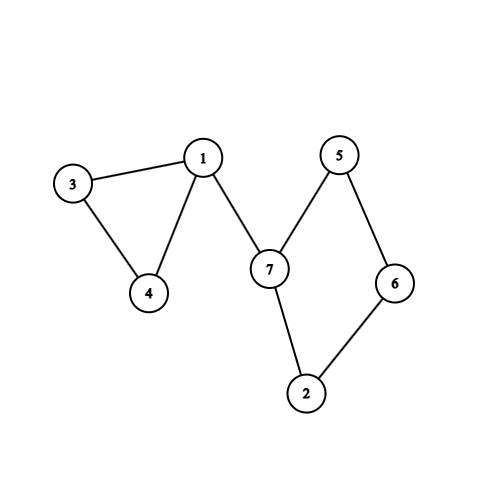
\includegraphics[width=0.2\textwidth]{resource/img/graph.png}
\end{figure}
\end{baitap}